% Emacs settings: -*-mode: latex; TeX-master: "manual.tex"; -*-

\section{Monochromator\_flat: An infinitely thin, flat mosaic crystal with 
a single scattering vector}
\label{s:monochromator_flat}

\component{Monochromator\_flat}{System}{$z_{\rm min}$, $z_{\rm max}$, $y_{\rm min}$, $y_{\rm max}$, $\eta_{\rm h}$, $\eta_{\rm v}$, $r_0$, $Q$}{$d_{\rm m}$}


This component simulates an infinitely thin single
crystal with a single scattering vector perpendicular to the
surface and a mosaic spread. A typical
use for this component is to simulate a simple monochromator or analyzer.

The physical model used in the component is a rectangular piece of
material composed of a large number of small micro-crystals.
The orientation of the
micro-crystals deviates from the nominal crystal orientation so that the
probability of a given micro-crystal orientation is proportional to a
Gaussian in the angle between the given and the nominal orientation. The
width of the Gaussian is given by the mosaic spread, $\eta$, of the crystal. 
$\eta$ is assumed to be large compared to the inherent Bragg width of the
scattering vector (often a few arc seconds).
The horizontal and vertical mosaicities, $\eta_{\rm h}$ and $\eta_{\rm v}$,
respectively, are allowed to be different.

The monochromator dimensions are given by the length, $z_{\rm w}$, and
the height, $y_{\rm h}$. As the parameter names indicate, the 
monochromator is initially placed in the $z-y$ plane. This definition
is made to ensure that the physical monochromator angle \verb+A1+ 
will equal the \MCS rotation angle around the $y$-axis.
 
As a further simplification, the crystal is assumed to be infinitely
thin. This means that multiple scattering effects are not simulated. It
also means that the total reflectivity is used as a parameter for
the model rather than the atomic scattering cross section, implying that
the scattering efficiency does not vary with neutron wavelength.
The variance
of the lattice spacing ($\Delta d/d$) is assumed to be zero, so this
component is not suitable for simulating backscattering instruments (use
the component {\rm Single\_crystal} 
in section~\ref{s:Single_crystal} for that).

When a neutron trajectory intersects the crystal, the first step in the
computation is to determine the probability of scattering. This
probability is then used in a Monte Carlo choice deciding whether to
scatter or transmit the neutron. The scattering probability is the sum
of the probabilities of first-order scattering, second-order, \ldots, up
to the highest order that permits Bragg scattering at the given neutron
wave length. However, in most cases at most one order will have a
significant scattering probability, and the computation thus considers
only the order that best matches the neutron wavelength. Bragg's law is
%
$$ n{\bf Q}_0 = 2{\bf k}_i\sin\theta $$
%
Thus, the scattering order is obtained simply as the integer multiple
$n$ of the nominal scattering vector ${\bf Q}_0$ which is closest to the
projection of $2{\bf k}_i$ onto ${\bf Q}_0$ (see
figure~\ref{f:mosaic_order}).
%  k=2PI/lambda
%  q=2k sin(theta)
%  
%  2 PI n/k = d q/2k
%  q = n 4 PI/d
%  
%  n 2PI/k = n 4 PI/q \sin\theta
%  1/k = 2/q\sin\theta
%  n q = 2k\sin\theta
\begin{figure}
  \begin{center}
    \psfrag{theta}[l][l]{$\theta$}
    \psfrag{ki}[r][r]{$2{\bf k}_{\rm i}$}
    \psfrag{Q0}[l][l]{${\bf Q}_0$}
    \psfrag{2Q0}[l][l]{$2{\bf Q}_0$}
    \psfrag{3Q0}[l][l]{$3{\bf Q}_0$}
    \psfrag{4Q0}[l][l]{$4{\bf Q}_0$}
    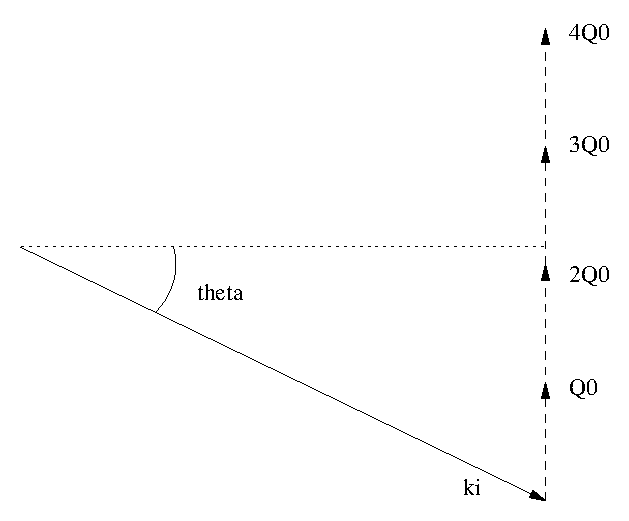
\includegraphics[width=0.5\textwidth]{figures/mosaic_order.eps}
  \end{center}
\caption{Selection of the Bragg order (``2'' in this case).}
\label{f:mosaic_order}
\end{figure}
%
Once $n$ has been determined, the Bragg angle $\theta$ can be
computed. The angle $d$ that the nominal scattering vector ${\bf Q}_0$
makes with the closest scattering vector ${\bf q}$ that admits Bragg
scattering is then used to compute the probability of reflection from
the mosaic
$$ p_{\rm reflect} = R_0 e^{-d^2/2\sigma^2}, $$
where $R_0$ is the reflectivity at the Bragg angle (see
figure~\ref{f:mosaic_angle}). The probability $p_{\rm reflect}$ is used
in a Monte Carlo choice to decide whether the neutron is transmitted or
reflected.
%
\begin{figure}
  \begin{center}
    \psfrag{th}[r][r]{$\theta$}
    \psfrag{ki}[r][r]{$2{\bf k}_{\rm i}$}
    \psfrag{kf}[l][l]{$2{\bf k}_{\rm f}$}
    \psfrag{Q0}[l][l]{${\bf Q}_0$}
    \psfrag{d}[c][c]{$d$}
    \psfrag{q}[l][l]{$\bf q$}
    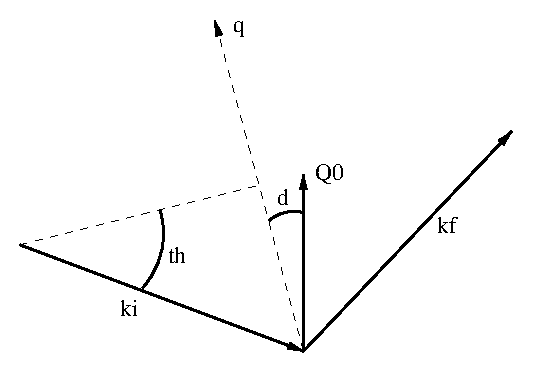
\includegraphics[width=0.5\textwidth]{figures/mosaic_angle.eps}
  \end{center}
\caption{Computing the deviation $d$ from the nominal scattering direction.}
\label{f:mosaic_angle}
\end{figure}

In the case of reflection, the neutron will be scattered into the
Debye-Scherrer cone, with the probability of each point on the cone
being determined by the mosaic. The Debye-Scherrer cone can be described
by the equation
\begin{equation}
  \label{eq:mosaic_cone}
  {\bf k}_{\rm f} = {\bf k}_{\rm i}\cos2\theta +
      \sin2\theta({\bf c}\cos\varphi + {\bf b}\sin\varphi),
      \qquad\varphi\in[-\pi;\pi],
\end{equation}
where ${\bf b}$ is a vector perpendicular to ${\bf k}_{\rm i}$ and ${\bf
Q}_0$, ${\bf c}$ is perpendicular to ${\bf k}_{\rm i}$ and ${\bf b}$,
and both ${\bf b}$ and ${\bf c}$ have the same length as ${\bf k}_{\rm
  i}$ (see figure~\ref{f:mosaic_cone}). When choosing $\varphi$ (and
thereby ${\bf k}_{\rm f}$), only a small part of the full $[-\pi; \pi]$
range will have appreciable scattering probability in non-backscattering
configurations. The best statistics is thus obtained by sampling
$\varphi$ only from a suitably narrow range.

The (small) deviation angle $\sigma$ of ${\bf q}$ from the nominal
scattering vector $n{\bf Q}_0$ corresponds to a $\Delta q$ of
$$ \Delta q \approx \sigma 2k\sin\theta. $$
The angle $\varphi$ corresponds to a $\Delta k_{\rm f}$ (and hence
$\Delta q$) of
$$ \Delta q \approx \varphi k \sin(2\theta) $$
(see figure~\ref{f:mosaic_cone}).
Hence we may sample $\varphi$ from a Gaussian with standard deviation
$$ \sigma\frac{2k\sin\theta}{k\sin(2\theta)} =
\sigma\frac{2k\sin\theta}{2k\sin\theta\cos\theta} =
\frac{\sigma}{\cos\theta} $$
to get good statistics.
%
\begin{figure}
  \begin{center}
    \psfrag{th}[r][r]{$2\theta$}
    \psfrag{ki}[c][c]{$2{\bf k}_{\rm i}$}
    \psfrag{kf}[r][r]{$2{\bf k}_{\rm f}$}
    \psfrag{nQ0}[l][l]{$n{\bf Q}_0$}
    \psfrag{q}[l][l]{$\bf q$}
    \psfrag{2ksin2t}[l][l]{$2 k \sin(2 \theta)$}
    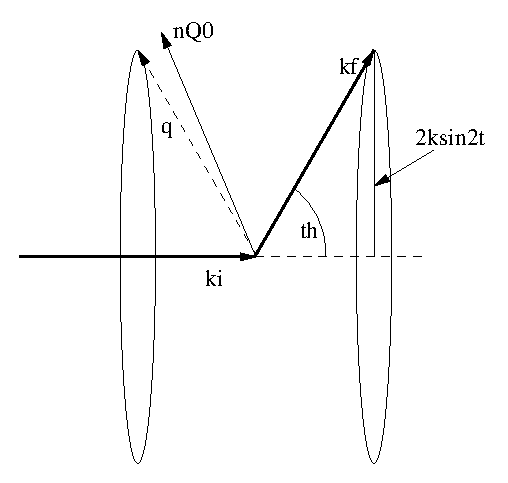
\includegraphics[width=0.5\textwidth]{figures/mosaic_cone.eps}
  \end{center}
\caption{Scattering into the part of the Debye-Scherrer cone covered by
    the mosaic.}
\label{f:mosaic_cone}
\end{figure}

What remains is to determine the neutron weight. The distribution from
which the scattering event is sampled is a Gaussian in $\varphi$ of
width $\frac{\sigma}{\cos\theta}$,
$$ f_{\rm MC}(\varphi) = \frac{1}{\sqrt{2\pi}(\sigma/\cos\theta)}
            e^{-\varphi^2/2(\sigma/\cos\theta)^2}
$$
In the physical model, the probability of the scattering event is
proportional to a Gaussian in the angle between the nominal scattering
vector ${\bf Q}_0$ and the actual scattering vector ${\bf q}$. The
normalization condition is that the integral over all $\varphi$ should
be 1. Thus the probability of the scattering event in the physical model
is
\begin{equation}
  \label{eq:mosaic_integral}
  \Pi(\varphi) = e^{\frac{-d(\varphi)^2}{2\sigma^2}} /
   \int_{-\pi}^{\pi} e^{\frac{-d(\varphi)^2}{2\sigma^2}} d\varphi
\end{equation}
where $d(\varphi)$ denotes the angle between the nominal scattering
vector and the actual scattering vector corresponding to $\varphi$.
According to equation~(\ref{probrule}), the weight adjustment $\pi_j$ is
then given by
$$ \pi_j = \Pi(\varphi) / f_{\rm MC}(\varphi). $$
In the implementation, the integral in~(\ref{eq:mosaic_integral}) is computed
using a 15-order Gaussian quadrature formula, with the integral
restricted to an interval of width $5\sigma/\cos\theta$ for the same
reasons discussed above on the sampling of $\varphi$.

The input parameters for Mosaic\_simple are \textit{zmin},
\textit{zmax}, \textit{ymin}, and \textit{ymax} to define the surface of
the crystal in the Y-Z plane; \textit{mosaic} to give the FWHM of the
mosaic spread; \textit{R0} to give the reflectivity at the Bragg angle,
and \textit{Qx}, \textit{Qy}, and \textit{Qz} to give the scattering
vector.

